\begin{block}{Homebrewing a Hybrid Solver}
    We design \texttt{QSplit}, a hybrid solver to increase the usage time of QPU.
    \texttt{QSplit} decomposes a QUBO problem into smaller QUBOS.
    \texttt{QSplit} relies on simple algebraic properties.

    \begin{figure}[h!]
        \centering
        \begin{minipage}{0.55\textwidth}
            Given any QUBO matrix we recursively divide it into four parts as in Figure \ref{fig:qubo}:
            \begin{enumerate}
                \item $\operatorname{ULs}$ and $\operatorname{BRs}$ are themselves QUBO matrices operating on a partition of the optimization variables;
                \item $\operatorname{UR}$ retains the information linking the partitions $\operatorname{UL}_0$ and $\operatorname{BR}_0$ of the variables and we can safely transform it into an upper triangular matrix, namely a QUBO instance;
                \item $\emptyset$ is a matrix composed entirely of zeros, so we ignore it.
            \end{enumerate}

            The recursive subdivision can continue until the matrices reach a predetermined size, namely the Stopping dimension.
        \end{minipage}%
        \hfill
        \begin{minipage}{0.4\textwidth}
            \centering
            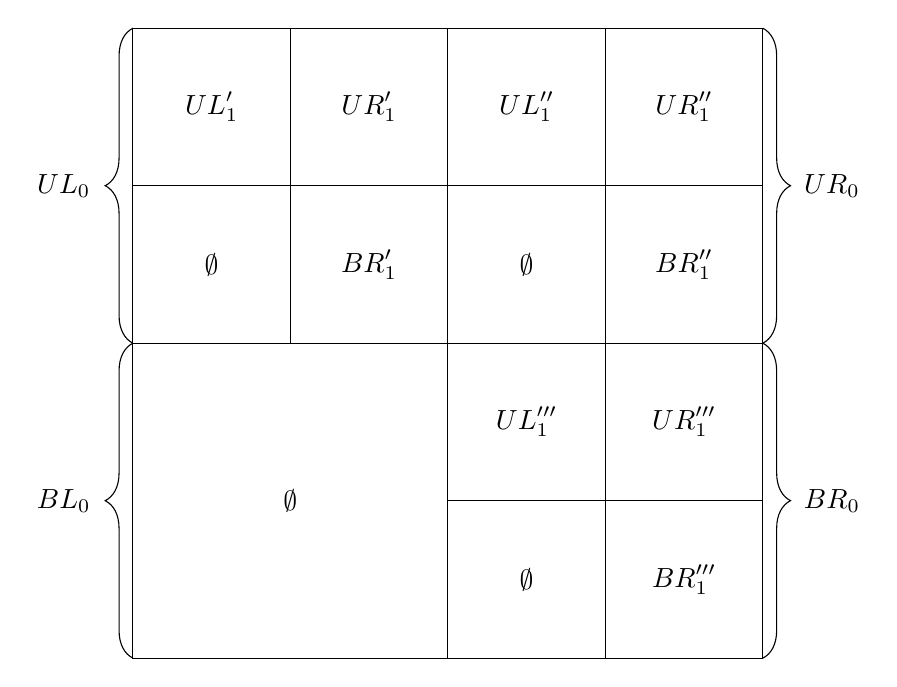
\begin{tikzpicture}
                \draw (0,0) rectangle (8,8);
            
                \draw (0,4) -- (8,4);
                \draw (4,0) -- (4,8);
                \node at (2,2) {$\emptyset$};
                
                \draw (0,6) -- (4,6);
                \draw (2,8) -- (2,4);
                \node at (1,5) {$\emptyset$};
            
                \draw (4,2) -- (8,2);
                \draw (6,4) -- (6,0);
                \node at (5,1) {$\emptyset$};

                \draw (4,6) -- (8,6);
                \draw (6,4) -- (6,8);
                \node at (5,5) {$\emptyset$};
            
                \draw[decorate,decoration={brace,amplitude=10pt}] (8,8) -- (8,4) node [black,midway,xshift=25pt] {$\operatorname{UR}_0$};
                \node at (3,7) {$\operatorname{UR}_1'$};
                \node at (7,7) {$\operatorname{UR}_1''$};
                \node at (7,3) {$\operatorname{UR}_1'''$};

                \draw[decorate,decoration={brace,amplitude=10pt,mirror}] (0,8) -- (0,4) node [black,midway,xshift=-25pt] {$\operatorname{UL}_0$};
                \node at (1,7) {$\operatorname{UL}_1'$};
                \node at (5,7) {$\operatorname{UL}_1''$};
                \node at (5,3) {$\operatorname{UL}_1'''$};

                \draw[decorate,decoration={brace,amplitude=10pt}] (8,4) -- (8,0) node [black,midway,xshift=25pt] {$\operatorname{BR}_0$};
                \node at (3,5) {$\operatorname{BR}_1'$};
                \node at (7,5) {$\operatorname{BR}_1''$};
                \node at (7,1) {$\operatorname{BR}_1'''$};

                \draw[decorate,decoration={brace,amplitude=10pt,mirror}] (0,4) -- (0,0) node [black,midway,xshift=-25pt] {$\operatorname{BL}_0$};
            \end{tikzpicture}
            \caption{Two steps of recursive decomposition}
            \label{fig:qubo}
        \end{minipage}
    \end{figure}

    \begin{exampleblock}{Example of one recursive step}
        Let us assume that we have classifications offered by $\operatorname{UL}_1'$, $\operatorname{UR}_1'$, $\operatorname{BR}_1'$. 

        \begin{enumerate}
            \item $\operatorname{UL}_1'$ and $\operatorname{BR}_1'$ are combined to generate conflict-free initial assignments called $\operatorname{S_1}$;
            \item The solutions from $\operatorname{S_1}$ and $\operatorname{UR}_1'$ are combined, and conflicting variables are marked;
            \item From the conflicting values, a QUBO problem is extracted, which is solved via QPU;
            \item From the set of possible assignments, the $k$ best distinct assignments are retained. 
        \end{enumerate}
    \end{exampleblock}
\end{block}